Effective decision-making 
requires choosing among options 
given the available information.
That much is unavoidable, 
unless we wish to make trivial decisions.
In selection processes, 
such as hiring, university admissions, and loan approval, 
the options are people;
the available features include 
(but are rarely limited to) 
direct evidence of qualifications;
and decisions impact lives. 

Laws in many countries restrict 
the ways in which certain decisions can be made.
For example,
Title VII of the US Civil Rights Act \cite{CivilRights1964},
forbids employment decisions that discriminate 
on the basis of certain \emph{protected characteristics}.
% \emph{race, color, religion, sex,} and \emph{national origin}.
Interpretation of this law 
has led to two notions of discrimination: 
\emph{disparate treatment} and \emph{disparate impact}.
%
%
\textit{Disparate treatment} 
addresses intentional discrimination, 
including 
(i) decisions explicitly based on protected characteristics; 
and (ii) intentional discrimination via proxy variables
(e.g~literacy tests for voting eligibility).
% to disenfranchise racial minorities).
%
\textit{Disparate impact}
addresses facially neutral practices
that might nevertheless
have an ``unjustified adverse impact 
on members of a protected class'' \cite{CivilRights1964}.  
One might hope that detecting unjustified impact were as simple as detecting unequal outcomes.
% (for some appropriate definition of outcome),
% or that such disparity could only arise through intentional discrimination.
However, absent intentional discrimination,
unequal outcomes can emerge due to correlations 
between protected and unprotected characteristics.
Complicating matters, unequal outcomes 
may not always signal unlawful discrimination \cite{AsianNYT}.

% While these legal doctrines are complex 
% and exceed the scope of this paper,
% we briefly summarize the relevant points:
% \textbf{Bringing forth a disparate impact case
% consists of multiple steps}. 
% The first step is to establish disparity 
% (by some measure) 
% in outcomes across groups,
% Subsequently, an employer must show 
% that the disparity arises 
% due to a business necessity.
% Joseph Seiner summarized the issue thusly
% in the Yale Law \& Policy Review:
% ``Confusion. 
% There is no better way to describe
% the current state of U.S. law 
% regarding allegedly discriminatory workplace standards'' 
% \cite{seiner2006disentangling}.
% As authors of a technical paper, 
% we will not presume to resolve longstanding debates
% among policy experts.
% % ZACK Not 100% satisfied, but better. note to revisit
% Our analysis will center on
% a line of papers on fairness in machine learning 
% and address the law only as it relates to 
% the claims and objectives of these papers.

% \alex{We're currently not distinguishing between the ML interpretation of disparate treatment and disparate impact and their legal interpretation.  This has us talking about criminal justice and admissions cases in the same paragraph as we're discussing disparate impact employment cases.  Whether disparate impact employment cases are difficult to prosecute is unrelated to the first part of this paragraph, and I think is unrelated to the arguments we're trying to make.  I've commented that bit out for now. }
% When a disparate impact employment case is prosecuted under Title VII,
% once the unequal outcomes are established,
% the burden falls to the defendant to
% ``demonstrate  that  the 
% challenged  practice  is  job  related  
% for  the  position  in  question  and  consistent 
% with business necessity''.
% The plaintiff might still win the case 
% by demonstrating a viable alternative with less disparate results \cite{CivilRights1964,barocas2016big}.
% As a practical matter, disparate impact cases are hard to win,
% so to some extent, mitigating disparate impact depends on non-compulsory policies. 

Recently, owing to the increased use
of machine learning (ML) 
to assist in consequential decisions,
the topic of quantifying and mitigating
ML-based discrimination 
has attracted interest 
% among both practitioners and academics 
in both policy and ML.
However, while the existing legal doctrine 
offers qualitative ideas,
%expressed in prose,
intervention in an ML-based system 
requires more concrete 
%mathematical 
formalism.
%
% While disparate treatment and disparate impact 
% are concepts rooted in United States anti-discrimination law,
% the topics have
%
%
%
%Loosely 
Inspired by the relevant legal concepts, technical papers have proposed several criteria 
to quantify discrimination. 
One criterion requires that 
the fraction given a positive decision be equal
across different groups.
Another criterion states that 
a classifier should be blind to the protected characteristic. Within the technical literature, these criteria are commonly referred to as \emph{disparate impact} and \emph{disparate treatment}, respectively.  


In this paper, we call these technical criteria \emph{impact parity} and \emph{treatment parity} 
to distinguish them from their legal antecedents.  
The distinction between 
technical and legal terminology 
is important to maintain. 
While impact and treatment parity 
are inspired by legal concepts, 
technical approaches that achieve these criteria 
may fail to satisfy 
the underlying legal and ethical desiderata. 
% Confusingly, \emph{disparate impact theory} and \emph{impact parity} are not the same.
% IP \emph{requires} having identical proportions of outcomes whereas in DI, group differences in outcome statistics are the first part 
% of a multi-step process.
% Likewise, \emph{disparate treatment} (which includes explicit proxy discrimination) and \emph{treatment parity} (which doesn't) are not the same.


% \textbf{In this paper}, we will call these technical criteria \emph{impact parity} (IP) and \emph{treatment parity} (TP), to distinguish them from their legal antecedents. 
% Confusingly, \emph{disparate impact theory} and \emph{impact parity} are not the same.
% IP \emph{requires} having identical proportions of outcomes whereas in DI, group differences in outcome statistics are the first part 
% of a multi-step process.
% Likewise, \emph{disparate treatment} (which includes explicit proxy discrimination) and \emph{treatment parity} (which doesn't) are not the same.
% Owing to this carelessness with language, 
% technical solutions motivated 
% by these definitions might fail to impact 
% the underlying legal and ethical desiderata 
% that they are designed to address.

We demonstrate one such disconnect
through DLPs,
a class of algorithms designed 
to simultaneously satisfy
treatment- and impact-parity criteria \cite{pedreshi2008discrimination,kamishima2011fairness,zafar2017fairness}.   
DLPs operate according to the following principle:
\emph{The protected characteristic may be used during training, but is not available to the model at prediction time.}
In the earliest such approach
the protected characteristic is used
to winnow the set of acceptable rules 
from an expert system \cite{pedreshi2008discrimination}.
Others incorporate the protected characteristic 
as either a regularizer, 
a constraint, 
or to preprocess the training data   \citep{kamiran2009classifying,kamiran2010discrimination,zafar2017fairness}.

These approaches are grounded in the premise 
that DLPs are acceptable in cases 
where using a protected characteristic 
as a direct input to the model
would constitute \emph{disparate treatment}
and thus be impermissible.  Indeed, DLPs in some sense operationalize a form of prospective fair ``test design'' that is well aligned with the ruling in \textit{Ricci v. DeStefano} \cite{kim2017auditing}.  
% We call this premise into question 
% on the following grounds:
In this paper we investigate the utility of DLPs as a technical solution
and present the following cautionary insights:
\begin{enumerate}
\item When protected characteristics 
are redundantly encoded in the other features, 
sufficiently powerful DLPs 
can (indirectly) implement any form of treatment disparity.
\item When protected characteristics are partially encoded
DLPs induce within-class discrimination 
based on irrelevant features,
and can harm some members of the protected group. 
\item DLPs provide a suboptimal trade-off 
between accuracy and impact parity. 
\item While disparate treatment is by definition illegal, 
the status of treatment disparity is debated \citep{kim2017data}.
% The optimal way to trade off the two 
% is to apply per-group thresholds, 
% effecting treatment disparity. 
\end{enumerate}

\begin{figure*}
\begin{center}
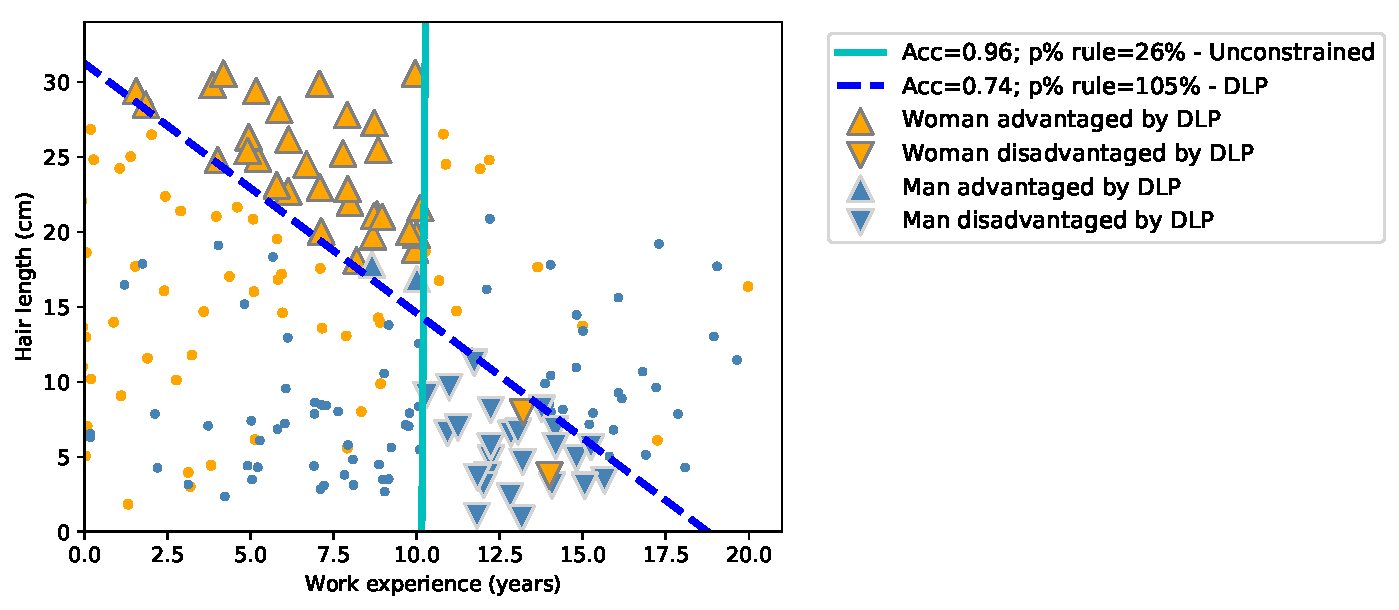
\includegraphics[width=.8\linewidth]{img/hair_workexp_new.pdf}
\end{center}
\caption{Demonstration of a DLP's undesirable side effects on a simple example of hiring data (see \S \ref{sec:synthetic}).  
An unconstrained classifier (vertical line)
hires candidates based on work experience,
yielding higher hiring rates for men than for women.  
A DLP (dashed diagonal) achieves near-parity 
by differentiating based on an irrelevant attribute (hair length).  
The DLP \emph{hurts} some short-haired women,
flipping their decisions to reject, 
and helps some long-haired men.
}
\label{fig:intragroup-disparity}
\end{figure*}

%JULIAN: Probably gotta go?
% The capacity of DLPs to carry out treatment disparity \emph{indirectly}
% casts doubt on whether, under the law,
% they would be viewed differently 
% from approaches that \emph{directly} apply treatment disparity.
% A recent California Law Review paper 
% \citep{grimmelmann2017incomprehensible} 
% supports this view, illustrating their
% arguments in the ``law-school hypothetical state" of Zootopia,
% where the protected groups are species.
% \begin{displayquote}
% In our view, Title VII does not permit an employer
% to do indirectly what it could not do directly. An employer that explicitly selects
% applicants on the basis of species violates Title VII under a disparate treatment theory, 
% regardless of whether species is correlated with job performance, 
% and regardless of whether it bears animus against particular species. It is the selection
% “on the basis of” species that is the problem. 
% An employer that uses home address to infer applicants’ species and then selects applicants from particular species
% does exactly the same, only in two steps rather than one. This too is a form of disparate treatment.
% \end{displayquote}
